% =====================================================================
%  N1: the generic block / link / source / constituent picture.
%  The governing form is Eq. (1) of Massoudieh (2023), EMS 164, 105707.
%
%  Build:  pdflatex fig_concept.tex && cp fig_concept.pdf figures/N1_block_link_concept.pdf
% =====================================================================
\documentclass[border=4pt]{standalone}
\usepackage[T1]{fontenc}
\usepackage{helvet}
\renewcommand\familydefault{\sfdefault}
\usepackage{amsmath}
\usepackage{tikz}
\usetikzlibrary{arrows.meta,positioning,calc,fit,backgrounds,decorations.pathmorphing}

\definecolor{ohqblue}{HTML}{1F5C8B}
\definecolor{ohqteal}{HTML}{2A9D8F}
\definecolor{ohqsand}{HTML}{E9C46A}
\definecolor{ohqrust}{HTML}{E76F51}
\definecolor{ohqgrey}{HTML}{6B7280}
\definecolor{water}{HTML}{BFD9E8}
\definecolor{panel}{HTML}{F3F6F8}

\begin{document}
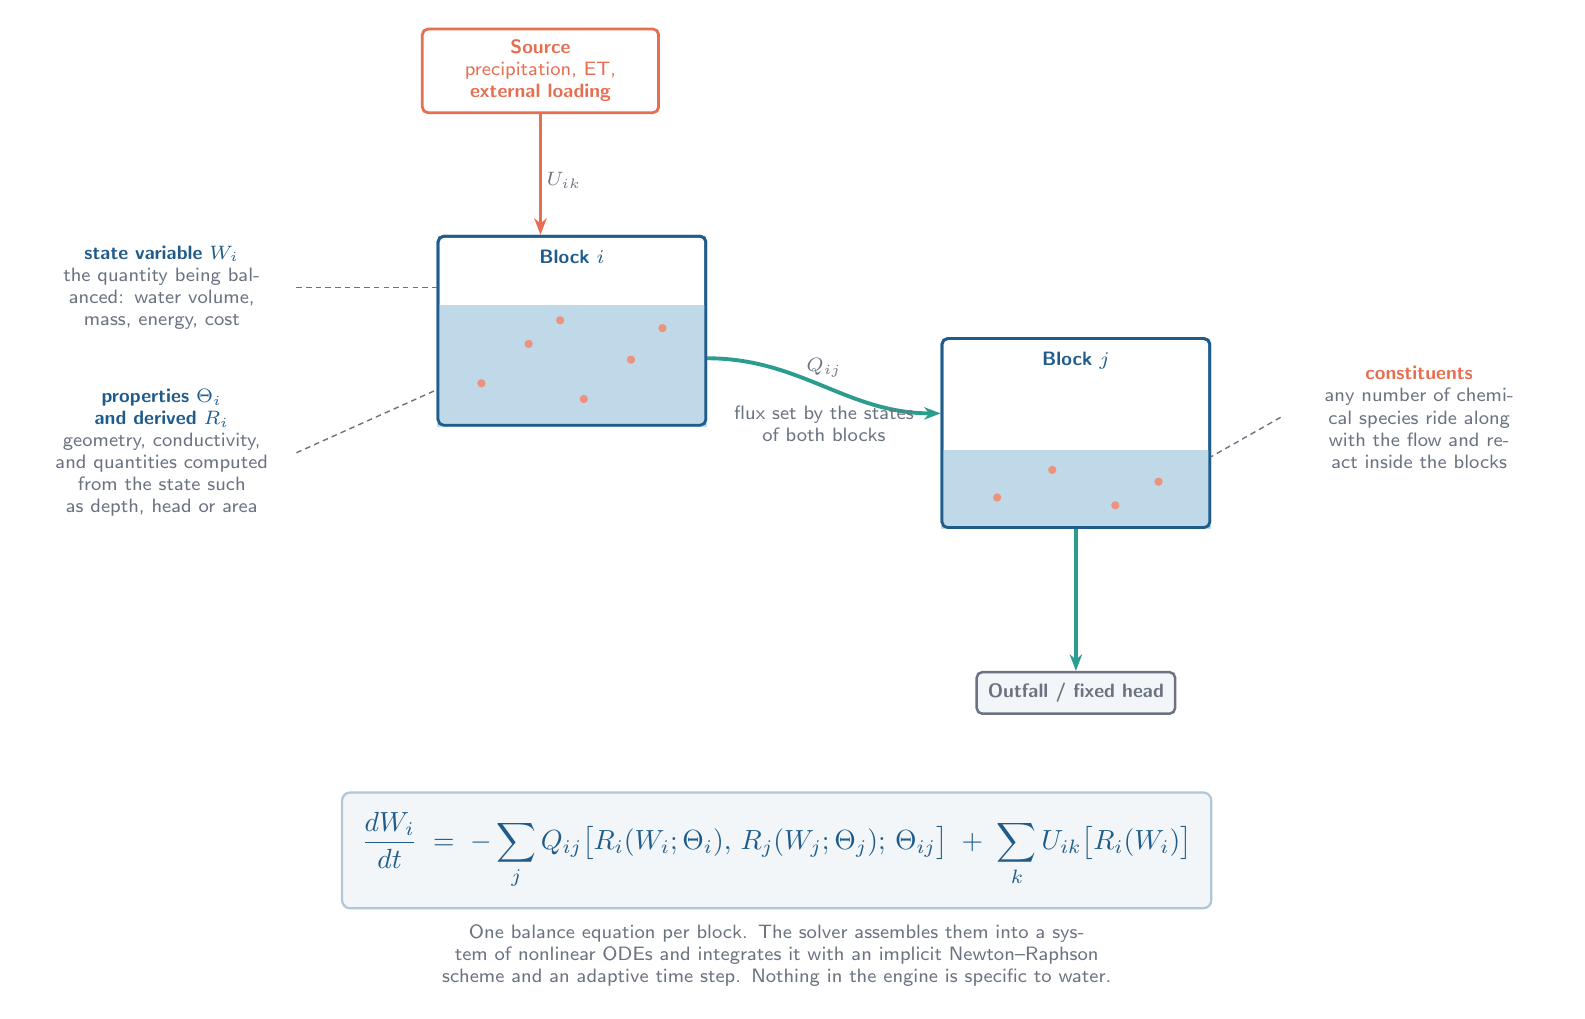
\begin{tikzpicture}[
  font=\sffamily,
  tank/.style={draw=ohqblue, line width=1pt, fill=white, rounded corners=2pt,
               minimum width=34mm, minimum height=24mm},
  flux/.style={-{Stealth[length=6pt]}, ohqteal, line width=1.4pt},
  src/.style={-{Stealth[length=6pt]}, ohqrust, line width=1.4pt},
  tag/.style={font=\scriptsize, text=ohqgrey, align=center, inner sep=1.5pt},
  key/.style={font=\scriptsize\bfseries, text=ohqblue, align=center},
  callout/.style={ohqgrey, line width=0.5pt, dashed, dash pattern=on 2pt off 1.5pt},
]

% ---------------- two blocks ---------------------------------------
\node[tank] (bi) at (0,0) {};
\node[tank] (bj) at (6.4,-1.3) {};

\begin{scope}
  \clip (bi.south west) rectangle (bi.north east);
  \fill[water] (bi.south west) rectangle ($(bi.south east)+(0,1.55)$);
  \foreach \x/\y in {-1.15/0.55, -0.55/1.05, 0.15/0.35, 0.75/0.85, 1.15/1.25, -0.15/1.35}
    \fill[ohqrust!75] ($(bi.south)+(\x,\y)$) circle (1.5pt);
\end{scope}
\begin{scope}
  \clip (bj.south west) rectangle (bj.north east);
  \fill[water] (bj.south west) rectangle ($(bj.south east)+(0,1.0)$);
  \foreach \x/\y in {-1.0/0.4, -0.3/0.75, 0.5/0.3, 1.05/0.6}
    \fill[ohqrust!75] ($(bj.south)+(\x,\y)$) circle (1.5pt);
\end{scope}
\node[tank, fill=none] at (0,0) {};
\node[tank, fill=none] at (6.4,-1.3) {};

\node[key, anchor=north] at ([shift={(0,-2pt)}]bi.north) {Block $i$};
\node[key, anchor=north] at ([shift={(0,-2pt)}]bj.north) {Block $j$};

% ---------------- source -------------------------------------------
\node[draw=ohqrust, line width=1pt, rounded corners=2pt, fill=white,
      font=\scriptsize\bfseries, text=ohqrust, align=center,
      minimum width=30mm, inner sep=4pt] (src) at (-0.4,3.3)
      {Source\\ \mdseries precipitation, ET,\\ external loading};
\draw[src] (src.south) -- node[tag, right, pos=0.55] {$U_{ik}$} ($(bi.north)+(-0.4,0)$);

% ---------------- links --------------------------------------------
\draw[flux] ($(bi.east)+(0,-0.35)$) to[out=0, in=180]
  node[tag, above, pos=0.5, yshift=1pt] {$Q_{ij}$}
  node[tag, below, pos=0.5, yshift=-5pt, text width=34mm]
    {flux set by the states\\of both blocks}
  ($(bj.west)+(0,0.25)$);

\node[draw=ohqgrey, line width=0.9pt, rounded corners=2pt, fill=panel,
      font=\scriptsize\bfseries, text=ohqgrey, inner sep=4pt,
      minimum width=22mm] (out) at (6.4,-4.6) {Outfall / fixed head};
\draw[flux] (bj.south) -- (out.north);

% ---------------- annotations --------------------------------------
\node[tag, anchor=east, text width=33mm] (ann1) at (-3.5,0.55)
  {\textbf{\textcolor{ohqblue}{state variable $W_i$}}\\
   the quantity being balanced: water volume, mass, energy, cost};
\draw[callout] (ann1.east) -- ($(bi.west)+(0,0.55)$);

\node[tag, anchor=east, text width=33mm] (ann2) at (-3.5,-1.55)
  {\textbf{\textcolor{ohqblue}{properties $\Theta_i$ and derived $R_i$}}\\
   geometry, conductivity, and quantities computed from the state such as
   depth, head or area};
\draw[callout] (ann2.east) -- ($(bi.west)+(0,-0.75)$);

\node[tag, anchor=west, text width=34mm] (ann3) at (9.0,-1.1)
  {\textbf{\textcolor{ohqrust}{constituents}}\\
   any number of chemical species ride along with the flow and react inside
   the blocks};
\draw[callout] (ann3.west) -- ($(bj.east)+(0,-0.3)$);

% ---------------- governing equation --------------------------------
\node[draw=ohqblue!35, line width=0.8pt, fill=panel, rounded corners=3pt,
      inner sep=7pt, text=ohqblue] (eq) at (2.6,-6.6)
  {$\displaystyle \frac{dW_i}{dt}
     \;=\; -\sum_j Q_{ij}\bigl[R_i(W_i;\Theta_i),\,R_j(W_j;\Theta_j);\,\Theta_{ij}\bigr]
     \;+\; \sum_k U_{ik}\bigl[R_i(W_i)\bigr]$};
\node[tag, anchor=north, text width=105mm] at ([shift={(0,-4pt)}]eq.south)
  {One balance equation per block. The solver assembles them into a system of
  nonlinear ODEs and integrates it with an implicit Newton--Raphson scheme and
  an adaptive time step. Nothing in the engine is specific to water.};

\end{tikzpicture}
\end{document}
